\section{Test}
\label{sec:test}
This chapter explains all the tests done on the new version of POP-C++ to be sure that this version is functional. The second part of this chapter is a report on the performance of the new version.


% ############################
%
% ----- BASIC FUNCTIONAL TESTS ---
%
% ############################
\subsection{Functional tests}
With the key exchange process, some functional tests have been made to verify the correct behaviour of this key exchange. This test are the same as the ones explained in the "User Manual" add-on.



% ############################
%
% ----- REAL SITUATION TESTS -----
%
% ############################
\subsubsection{Real situation test}
To prove our theory, a real test situation has been put in place at EIA-FR. This section will explain the infrastructure and the constraints of this situation. \s

\textbf{\textit{TODO}}: if test with Geneva done, include all the details. \s

\textbf{EIA-FR test infrastructure}\\
The GRID \& Cloud Computing Group has got a DMZ that can be managed without the intervention of the IT Head Office of the school. This DMZ is delimited from the Internet by a firewall (FW). This FW is able to manage different areas. These areas are working as different networks. Nowadays, four different areas are in place. 

\begin{itemize}
\item "Grille Collaborateurs" - Collaborators GRID
\item "Grille étudiants" - Students GRID
\item "Servers"
\item "Grille Test" - Test GRID
\end{itemize}

Figure \ref{fig:eia_dmz} shows the current configuration of the EIA-FR DMZ

\begin{figure}[ht]
	\caption{EIA-FR DMZ}
  	\centering
	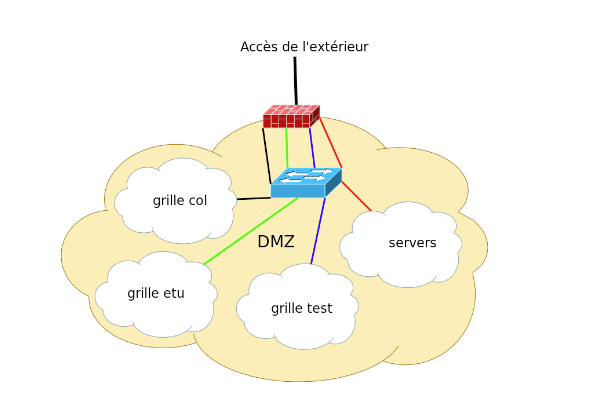
\includegraphics[scale=0.6]{./pic/dmz1.png}
	\label{fig:eia_dmz}
\end{figure}

The subnet 160.98.22.0/23 is available for the computers located in the DMZ. \s

\textbf{Restriction}\\
The only restriction imposed by the IT Head Office is to block the SMPT port (25) and the SMPT-S port (587). This restriction avoid the unwanted use of a mail server installed in the DMZ as a routing server for SPAM. This problem could put the all school network (160.98.0.0) to be on a blacklist. \s

\textbf{Area}\\
The IP address range 160.98.22.1 to 160.98.22.254 is subdivided as follows:

\begin{center}
\begin{tabular}{|p{2.5cm}|p{2.5cm}|p{2.5cm}|p{2.5cm}|}
\hline
\textbf{Area} & \textbf{Subnet}	& \textbf{Gateway} & \textbf{Mask}\\ \hline
Grille étudiants & 160.98.22.0 & 160.98.22.1 & 255.55.255.192 \\ \hline
Grille collaborteurs & 160.98.22.64 & 160.98.22.65 & 255.55.255.192 \\ \hline
Grille test & 160.98.22.128 & 160.98.22.129 & 255.55.255.192 \\ \hline
Servers & 160.98.22.192 & 160.98.22.193 & 255.55.255.192 \\ \hline
\end{tabular}
\end{center}\s

Rules have been globally defined for each area. Some specific rules are defined for well defined computers. 

\textbf{Proposition for the ViSaG project}\\
To avoid external access to the internal school network, the school network is simulated by an area in the DMZ. \s

A computer named "Master1", in the rest of this section, will be installed in the area "Grille collaborateur". In the ViSaG project, this computer will be the only access point for HEPIA and HE-Arc. \s

A second computer named "Master2" will be installed in the area "Grille Test". This computer will be accessible by Master1. Master1 and Master2 are physical computer running VMware ESXi.\s

On these computers, a virtual machine (VM) named "Admin" will run permanently. The "Admin" VM on Master1 and the one on Master2 will be able to communicate together because they made the confidence link.
When a request is coming on one "Admin" VM, a "Worker" VM is launched. The computation work will be done in these "Worker" VMs.\s

\pagebreak
A DHCP server need to be set to give IP Address to the "Worker" VM. As shown on Figure \ref{fig:dmz_dhcp1}, the DHCP server will be installed on an "Admin" VM. The IP address distributed by the DHCP server must be public address.

\begin{figure}[ht]
	\caption{DHCP server on "Admin"}
  	\centering
	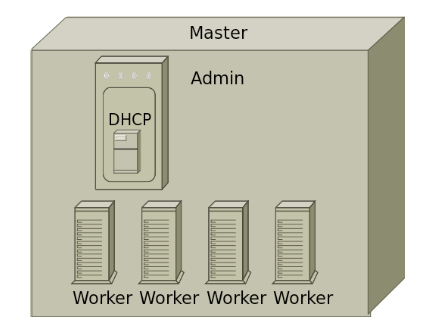
\includegraphics[scale=0.6]{./pic/dmz2.png}
	\label{fig:dmz_dhcp1}
\end{figure}

The DHCP server could also be set on an external VM as shown on Figure \ref{fig:dmz_dhcp2}.

\begin{figure}[ht]
	\caption{DHCP server on an external VM}
  	\centering
	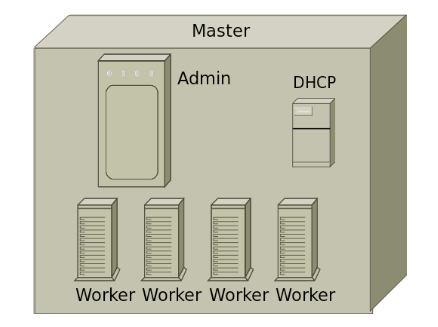
\includegraphics[scale=0.6]{./pic/dmz3.png}
	\label{fig:dmz_dhcp2}
\end{figure}

\textbf{Important point}\\
It is important than only one DHCP server is accessible in an area. The FW will be configured to communicate with a specific computer with a specific IP address. If the "Worker" get his IP address from another DHCP server, this address will be blocked by the FW.\s

In order that the "Worker" managed by the "Admin" on Master1 can communicate with the "Worker" managed by the "Admin" on Master2, the port 22 (SSH) must be open for the IP address attibuted to the "Worker". A number of rules egal to the number of "Worker" + 2 ("Master" + "Admin") must be defined on the FW. To avoid to many rules on the FW, the DHCP server will be configured to attribute only the good number of IP address for the "Worker" VM. \s

\begin{figure}[ht]
	\caption{Logical View of the infrastructure}
  	\centering
	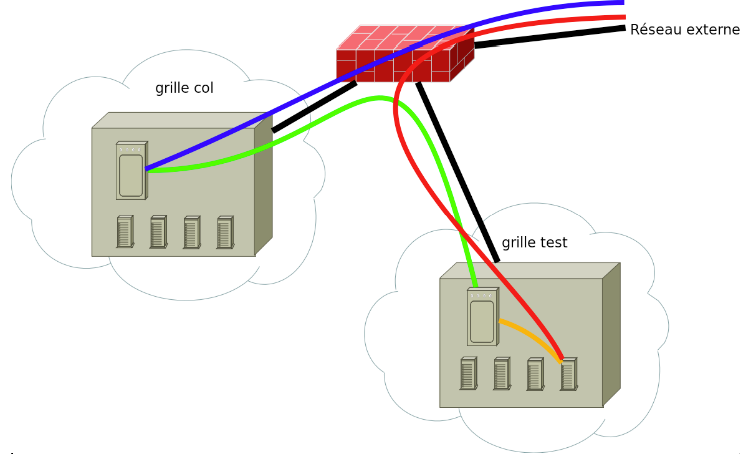
\includegraphics[scale=0.6]{./pic/dmz4.png}
	\label{fig:logical_dmz}
\end{figure}

Figure \ref{fig:logical_dmz} shows a logical view of the DMZ with our two different area working as two different network separated by a FW. The different link color represents: 

\begin{itemize}
\item Black: physical connection
\item Blue: connection on the "Admin" VM
\item Green: Communication between JobMgr
\item Orange: "Worker" creation
\item Red: Communication between "Worker" and the POP-C++ application
\end{itemize}

% ############################
%
% ----- PERFORMANCE TESTS -----
%
% ############################
\subsection{Performance tests}
We were aware that using virtual machine and secure connection will affect the performance of POP-C++. To know which part of the execution is the slowest compared to the standard version, some performance tests have been made. This section explains the different test case and the results.

\subsubsection{Matrix Computation with POP-C++ Standard Version}
To have a basis, we first made performance test on the same architecture but with the Standard version of POP-C++. This section reports all the measures and the results. \s

\textbf{Infrastructure}\\
The infrastructure is composed by three Virtual Machines running on three different ESXi platforms. Each VM have a standard version of POP-C++ installed. The configuration of the global services is made to share the charge between the three nodes. \s

\textbf{Measurements}\\
As the infrastructure for the POP-C++ VS is small, the test for the standard basis version must be done on the same small infrastructure of three nodes. The tests have been performed with three different matrix size and for each matrix size, three different numbers of workers.
\begin{center}
\begin{tabular}{|p{3cm}|p{3cm}|p{3cm}|}
\hline
\textbf{Matrix Size} & \textbf{Nb Workers}	& \textbf{Nb workers/VM} \\ \hline
600x600 & 1 & 1\\ \hline
600x600 & 3 & 1\\ \hline
600x600 & 6 & 2\\ \hline
600x600 & 9 & 3\\ \hline
900x900 & 1 & 1\\ \hline
900x900 & 3 & 1\\ \hline
900x900 & 6 & 2\\ \hline
900x900 & 9 & 3\\ \hline
1200x1200 & 1 & 1\\ \hline
1200x1200 & 3 & 1\\ \hline
1200x1200 & 6 & 2\\ \hline
1200x1200 & 9 & 3\\ \hline
\end{tabular}
\end{center}\s


\subsubsection{Matrix Computation with POP-C++ standard version}
To have a basis for the performance tests on POP-C++ VS, we have run the same tests on the same architecture but with the POP-C++ standard version. This section details the result of these executions. \s

\textbf{Speedup}\\
The speedup has been computed with the different result obtained 
\begin{center}
\begin{tabular}{|p{6cm}|p{2cm}|p{2cm}|p{2cm}|p{2cm}|}
\hline
\textbf{Matrix Size/Nb of workers} & \textbf{1}	& \textbf{3} 	& \textbf{6}	& \textbf{10}\\ \hline
\textbf{600x600} &5.17748 & 2.1383 &	2.3859	& 2.7290 \\ \hline
\textbf{900x900} &16.4920&	6.1572&	6.5519	&7.5837\\ \hline
\textbf{1200x1200} &38.5506 & 13.9942	 & 14.5949 & 16.7564\\ \hline

\end{tabular}
\end{center}\s

\begin{figure}[ht]
	\caption{Speedup for POP-C++ Standard execution}
  	\centering
	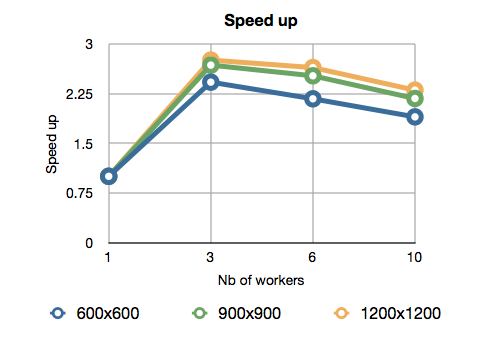
\includegraphics[scale=0.6]{./pic/speedup_std.png}
	\label{fig:speedup1}
\end{figure}

\subsubsection{Matrix Computation with POP-C++ Virtual-Secure version}



